\subsection{ТЕОРЕТИЧЕСКОЕ ОПИСАНИЕ ГЭЦ В РАМКАХ СТОЛБЧАТОЙ МОДЕЛИ}

В данном разделе будет приведен вывод основных соотношений, описывающих такие параметры ГЭЦ, как ИП и ГП. При этом будет использована столбчатая модель. Отличительной чертой класса столбчатых моделей ГЭЦ является разделение слоя воздуха между поверхностью Земли и ионосферой на столбцы воздуха, в каждом из которых задачу полагают одномерной. Более подробно столбчатая модель будет описана ниже (см. раздел \ref{sec:stolb}).

\subsubsection{ФОРМУЛИРОВКА ЗАДАЧИ В ТЕРМИНАХ ПОЛЕЙ}

Ниже символом $\Omega$ (см. рис. \ref{fig:gec-scheme}{a}) будет обозначаться область атмосферы, ограниченную поверхностью Земли $\Gamma_1$ и некоторой поверхностью $\Gamma_2$, лежащей в нижней ионосфере. Уравнения Максвелла в гауссовой системе единиц для напряженности магнитного поля $\vb{H}(\vb{r},\, t)$, индукции магнитного поля $\vb{B}(\vb{r},\, t)$, напряженности электрического поля $\vb{E}(\vb{r},\, t)$ и индукции электрического поля $\vb{D}(\vb{r},\, t)$ запишутся следующим образом:
\begin{equation}
    \curl{\vb{H}} = \dfrac1c \pdv{\vb{D}}{t} + \dfrac{4\pi}{c}\vb{j},
    \label{eq:1}
\end{equation}
\begin{equation}
    \curl{\vb{E}} = -\dfrac1c \pdv{\vb{H}}{t},
    \label{eq:2}
\end{equation}
\begin{equation}
    \div{\vb{B}} = 0,
    \label{eq:3}
\end{equation}
\begin{equation}
    \div{\vb{D}} = 4\pi\rho,
    \label{eq:4}
\end{equation}
где $\vb{j}(\vb{r},\, t)$ --- плотность электрического тока, $\rho(\vb{r},\, t)$ --- плотность электрического заряда. В качестве материальных соотношений будут использоваться выражения: 
\begin{equation}
    \vb{B} = \vb{H},\; \vb{D} = \vb{E},\; \vb{j} = \sigma \vb{E} + \vb{j}_s,
\end{equation}
где $\sigma(\vb{r},\, t)$ --- проводимость, $\vb{j}_\mathrm{s}(\vb{r},\, t)$ --- плотность тока источников (sources). Используя такие соотношения, в стационарном приближении ($\pdv*{\vb{H}}{t} = \pdv*{\vb{D}}{t} = 0$) уравнения Максвелла \eqref{eq:1}--\eqref{eq:4} можно переписать в следующем виде:
\begin{equation}
    \curl{\vb{H}} = \dfrac{4\pi}{c}\qty(\sigma \vb{E} + \vb{j}_s),
    \label{eq:5}
\end{equation}
\begin{equation}
    \curl{\vb{E}} = 0,
    \label{eq:6}
\end{equation}
\begin{equation}
    \div{\vb{H}} = 0,
    \label{eq:7}
\end{equation}
\begin{equation}
    \div{\vb{E}} = 4\pi\rho.
    \label{eq:8}
\end{equation}

\begin{figure}[htbp]
    \centering
    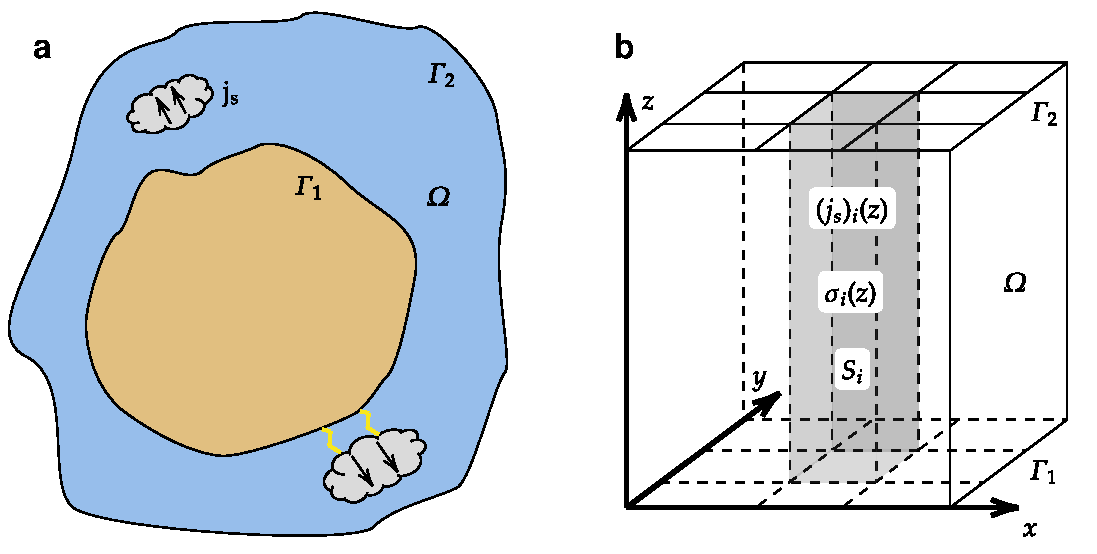
\includegraphics[width=\textwidth]{figures/gec-scheme.pdf}
    \caption{(a): Схематичное изображение ГЭЦ. (b): Иллюстрация к столбчатой модели ГЭЦ.}
    \label{fig:gec-scheme}
\end{figure}

Важно заметить, что проводимость Земли превышает проводимость приповерхностного воздуха на несколько порядков \cite[Рис. 1]{Mareev_2010}, что позволяет положить поверхность Земли $\Gamma_1$ идеально проводящей. Кроме того, следует отметить, что проводимость воздуха экспоненциально увеличивается с высотой \cite[Рис. 1]{Mareev_2010}, что позволяет считать и поверхность $\Gamma_2$ идеально проводящей, если она достаточно удалена от $\Gamma_1$ (так далеко, чтобы проводимость воздуха достигла величин, сопоставимых с проводимостью поверхности Земли, обычно это $\sim 70\, \textnormal{км}$). Такие рассуждения приводят к граничным условиям на тангенциальную компоненту электрического поля
\begin{equation}
    E_\tau \eval_{\Gamma_1} = 0,\; E_\tau \eval_{\Gamma_2} = 0.
    \label{eq:gu_pol}
\end{equation}

Таким образом, уравнения \eqref{eq:5} и \eqref{eq:6} c граничными условиями \eqref{eq:gu_pol} позволяют по заданным источникам $\vb{j}_s(\vb{r})$ и проводимости $\sigma(\vb{r})$ найти поля $\vb{E}(\vb{r})$ и $\curl{\vb{H}(\vb{r})}$.

\subsubsection{ФОРМУЛИРОВКА ЗАДАЧИ В ТЕРМИНАХ ПОТЕНЦИАЛА}

Из уравнения \eqref{eq:6} следует возможность введения потенциала, то есть такой функции $\varphi(\vb{r})$, что 
\begin{equation}
    \vb{E} = - \grad{\varphi}.
    \label{eq:11}
\end{equation}
Граничные условия \eqref{eq:gu_pol} для потенциала $\varphi(\vb{r})$ можно переписать в виде
\begin{equation}
    \varphi\eval_{\Gamma_1} = 0,\; \varphi\eval_{\Gamma_1} = V,
    \label{eq:gu_pot}
\end{equation}
где $V=\mathrm{const}$ --- ионосферный потенциал, который полагается неизвестной константой и находится в ходе решения задачи.

На потенциал $\varphi(\vb{r})$ можно записать следующую систему уравнений:
\begin{equation}
    \div{\qty(- \sigma \grad{\varphi} + \vb{j}_s)} = 0,
    \label{eq:13}
\end{equation}
\begin{equation}
    \oint\limits_{\Gamma_1} \qty(- \sigma \grad{\varphi} + \vb{j}_s) \dd{\vb{s}} = 0.
    \label{eq:14}
\end{equation}
Такие уравнения вместе эквивалентны уравнению \eqref{eq:5}. Действительно, векторное поле $\vb{X}$ может быть записано в виде ротора некоторого поля $\vb{Y}$ в области $\Omega$ тогда и только тогда, когда одновременно выполняется два условия: $\div{\vb{X}} = 0$ и равен нулю поток поля $\vb{X}$ через поверхность $\Gamma_1$ или $\Gamma_2$. При этом поле $\vb{Y}$ получается неопределенным с точностью до градиента некоторой функции $\chi$%, то есть всегда можно подобрать такое $\chi$, чтобы занулить $\div{\vb{Y}}$.
. Если возвращаться от общих рассуждений к конкретике, то в настоящем случае роль $\vb{X}$ играет векторное поле $- \sigma \grad{\varphi} + \vb{j}_s$, а роль $\vb{Y}$ --- напряженность магнитного поля $\vb{H}$, как видно из \eqref{eq:5}. Важно заметить, что уравнения \eqref{eq:13} и \eqref{eq:14} не только эквивалентны уравнению \eqref{eq:5}, но и не противоречат уравнению \eqref{eq:7} (которому можно удовлетворить, пользуясь тем, что $\vb{H}$ получается неопределенным с точностью до градиента некоторой функции $\chi$, которую всегда можно выбрать таким образом, чтобы удовлетворить \eqref{eq:7}).

Таким образом, для нахождения потенциала электрического поля $\varphi(\vb{r})$ при заданных источниках $\vb{j}_s(\vb{r})$ и проводимости $\sigma(\vb{r})$ требуется решить уравнения \eqref{eq:13} и \eqref{eq:14} с граничным условием \eqref{eq:gu_pot}. Корректность такой задачи обсуждается в \cite{Kalinin_et_al_2014}.

\subsubsection{ФОРМУЛИРОВКА ЗАДАЧИ НА ПОТЕНЦИАЛ В РАМКАХ СТОЛБЧАТОЙ МОДЕЛИ}
\label{sec:stolb}

В рамках столбчатой модели ГЭЦ поверхности $\Gamma_1$ и $\Gamma_2$ полагаются плоскостями, расположенными ортогонально оси высот $z$ (см. рис. \ref{fig:gec-scheme}{b}; обоснованность такого подхода будет обсуждена ниже в разделе \ref{sec:obosn}), при этом можно считать, что ось $x$, например, долготам, а ось $y$ --- широтам. Поверхностям $\Gamma_1$ и $\Gamma_2$ соответствуют высоты $z=0$ и $z=H_0$. Область атмосферы $\Omega$, которая теперь имеет форму прямоугольного параллелепипеда, разбивается на не перекрывающиеся цилиндры (столбцы) с образующими, параллельными оси высот $z$. В каждом столбце потенциал $\varphi(\vb{r})$ полагается изменяющимся лишь вдоль оси высот $z$, то есть $\pdv*{\varphi}{x} = \pdv*{\varphi}{y} = 0$ внутри каждого отдельного столбца. Таким образом, если в исходной постановке задачи потенциал $\varphi(\vb{r})$ был непрерывной функцией точки в области $\Omega$, то при переходе к столбчатой модели сохраняется лишь непрерывная зависимость потенциала от высоты $z$, а зависимость от поперечных координат дискретизируется и переходит в зависимость потенциала от номера столбца.

В рамках рассматриваемого приближения уравнения \eqref{eq:13} и \eqref{eq:14} принимают вид
\begin{equation}
    \dv{z}\qty(\sigma_i(z)\dv{\varphi_i}{z}\qty(z) - \qty(j_\mathrm{s})_i\qty(z)) = 0,\; i=\overline{1,\, N},
    \label{eq:15}
\end{equation}
\begin{equation}
    \sum\limits_{i=1}^{N} \qty(\sigma_i(z)\dv{\varphi_i}{z}\qty(z) - \qty(j_\mathrm{s})_i\qty(z))\cdot S_i = 0,
    \label{eq:16}
\end{equation}
где $i$ --- номер столбца, $S_i$ --- площадь основания столбца, $\qty(j_\mathrm{s})_i\qty(z)$ --- проекция тока источников в $i$-ом столбце на ось высот $z$. Следует заметить, что уравнение \eqref{eq:13} переходит в уравнение \eqref{eq:15} в рамках столбчатой модели, только если пренебречь поперечными токами, то есть $(\vb{j}_\mathrm{s})_{\perp} = 0$. Такое приближение хорошо работает в ГЭЦ из-за значительной разнице в двух пространственных масштабах: поперечный размер ГЭЦ сильно больше вертикального (поэтому токи в основном текут вдоль вертикали, по пути наименьшего сопротивления). Уравнение \eqref{eq:15} означает постоянство величины $\sigma_i(z)\dv*{\varphi_i}{z}\qty(z) - \qty(j_\mathrm{s})_i\qty(z)$ внутри $i$-ого столбца, что в свою очередь позволяет распространить \eqref{eq:14} с $\Gamma_1$ на любую поверхность между $\Gamma_1$ и $\Gamma_2$ и получить \eqref{eq:16}. Граничные же условия \eqref{eq:gu_pot} перейдут в следующие условия:
\begin{equation}
    \varphi_i\qty(z=0) = 0,\;  \varphi_i\qty(z=H_0) = V,\; i=\overline{1,\, N},
    \label{eq:gu_pot_stolb}
\end{equation}
где $V = \mathrm{const}$ --- ионосферный потенциал, полагаемый в ходе решения задачи неизвестной константой.

В итоге в рамках столбчатой модели ГЭЦ уравнения \eqref{eq:15} и \eqref{eq:16} с граничными условиями \eqref{eq:gu_pot_stolb} позволяют найти потенциал электрического поля $\varphi(\vb{r})$, если в каждом из $N$ столбцов модели заданы высотные профили проводимости $\sigma_i\qty(z)$ и плотности тока источников $\qty(j_\mathrm{s})_i\qty(z)$, а так же площади оснований $S_i$.

\subsubsection{АНАЛИТИЧЕСКОЕ РЕШЕНИЕ ЗАДАЧИ В РАМКАХ СТОЛБЧАТОЙ МОДЕЛИ}

Для решения задачи удобно ввести ток
\begin{equation}
    I_i (z) = \qty(\qty(j_\mathrm{s})_i\qty(z) - \sigma_i(z)\dv{\varphi_i}{z}\qty(z)) \cdot S_i,\; i=\overline{1,\, N}.
    \label{eq:I_i}
\end{equation}
Важно заметить, что из уравнения \eqref{eq:15} следует, что величины $I_i$ не зависят от высоты $z$ и являются постоянными для каждого отдельного столбца модели. 

Из определения \eqref{eq:I_i} можно выразить 
\begin{equation}
    \dv{\varphi_i}{z}\qty(z) = \dfrac{\qty(j_\mathrm{s})_i\qty(z) - I_i / S_i}{\sigma_i(z)},\; i=\overline{1,\, N},
\end{equation}
а затем проинтегрировать по высоте $z$ от $z=0$ до $z=z'$, что приведет к соотношению
\begin{equation}
    \varphi_i(z)\eval_{0}^{z'} = \int\limits_{0}^{z'} \dfrac{(j_\mathrm{s})_i}{\sigma_i} \dd{z} - \dfrac{I_i}{S_i} \int\limits_{0}^{z'} \dfrac{1}{\sigma_i} \dd{z}.
    \label{eq:phi}
\end{equation}
Если в качестве верхнего предела интегрирования положить высоту второй поверхности $\Gamma_2$, то есть $z'=H_0$, то из \eqref{eq:phi} получается выражение ИП
\begin{equation}
    V = \varphi_i(z)\eval_{0}^{H_0} = \int\limits_{0}^{H_0} \dfrac{(j_\mathrm{s})_i}{\sigma_i} \dd{z} - \dfrac{I_i}{S_i} \int\limits_{0}^{H_0} \dfrac{1}{\sigma_i} \dd{z}.
    \label{eq:21}
\end{equation}
Данное выражения для ИП не является конечным, так как в нем присутствует неизвестная величина $I_i$, ее следует исключить. Для этого надо воспользоваться уравнением \eqref{eq:16}, которое равноценно условию $\sum_{i=1}^N I_i = 0$. Если выразить из \eqref{eq:21} ток $I_i$ и просуммировать получившееся выражение по всем $i$, то удастся прийти к следующему выражению для ИП:
\begin{equation}
    V = \sum\limits^N_{i=1}\qty(S_i \int\limits_0^{H_0} \dfrac{(j_\mathrm{s})_i}{\sigma_i} \dd{z} \Bigg/
    \int\limits_0^{H_0} \dfrac{\dd{z}}{\sigma_i})
    \Bigg/
    \sum\limits^N_{i=1}\qty( S_i \Bigg/ {\int\limits_0^{H_0} \dfrac{\dd{z}}{\sigma_i}}).
    \label{eq:ip_stolb}
\end{equation}

Кроме того, возможно получить выражение и на высотный профиль потенциала $\varphi_i(z)$. Для этого следует подставить в \eqref{eq:phi} граничное условие на $\Gamma_1$ и выражение для $I_i$ через ИП, которое возможно получить из \eqref{eq:21}. Тогда не трудно видеть, что высотный профиль потенциала будет даваться выражением
\begin{equation}
    \varphi_i (z) = \int\limits_{0}^{z} \dfrac{(j_\mathrm{s})_i}{\sigma_i} \dd{z} - \qty[\int\limits_{0}^{z} \dfrac{\dd{z}}{\sigma_i} \Bigg/ \int\limits_{0}^{H_0} \dfrac{\dd{z}}{\sigma_i}]\times \qty(\int\limits_{0}^{H_0} \dfrac{(j_\mathrm{s})_i}{\sigma_i} \dd{z} - V),
    \label{eq:phi_stolb}
\end{equation}
где ионосферный потенциал $V$ определяется из формулы \eqref{eq:ip_stolb}. Отсюда можно получить выражение для ГП в регионе хорошей погоды. Для этого следует заметить, что под регионом хорошей погоды понимается столбец без источников, то есть $(j_\mathrm{s})_i=0$ в данном столбце. Тогда дифференцирование по высоте выражения \eqref{eq:phi_stolb} дает следующее выражение для приповерхностного ГП в регионе хорошей погоды:
\begin{equation}
\label{eq:pg_ip}
    \pdv{\varphi_i}{z} \qty(z=0) = \dfrac{V}{\sigma_i(z=0)} \qty(\int\limits_{0}^{H_0} \dfrac{\dd{z}}{\sigma_i(z)})^{-1}.
\end{equation}
Данное соотношение связывает ИП и приповерхностный ГП, измеренный в хорошую погоду.

Таким образом решается задача на потенциал электрического поля в рамках столбчатой модели ГЭЦ. Формулы \eqref{eq:ip_stolb} и \eqref{eq:phi_stolb} позволяют по заданным проводимости, плотности тока источников и площадям оснований столбцов найти ИП и профиль потенциала в каждом из столбцов.

\subsubsection{ОБОСНОВАННОСТЬ ИСПОЛЬЗОВАНИЯ СТОЛБЧАТОЙ МОДЕЛИ}
\label{sec:obosn}
% В данном разделе будет рассмотрен вопрос о том, насколько обоснованны предположения, на которых строится столбцовая модель ГЭЦ. 

% привести формулу для ИП, полученную в рамках сферической модели и сравнить ее с той, что получилась в рамках столбчатой модели. Прийти к выводу, что формулы различаются незначительно.

В рамках столбчатой модели ГЭЦ атмосфера описывается как набор параллельных не перекрывающихся столбцов, внутри которых токи полагаются текущими строго вдоль вертикали, что безусловно является идеализацией. Пренебречь поперечной структурой токов можно из-за того, что поперечный масштаб ГЭЦ значительно превышает ее характерный вертикальный масштаб, а токи в основном текут вдоль пути наименьшего сопротивления --- вдоль нормали между двумя эквипотенциальными плоскостями.

Ниже будет обоснован переход от сложной формы поверхности Земли к плоской геометрии. Стандартным приближением при исследовании Земли является аппроксимация формы поверхности Земли сферой, следовательно, логично положить поверхности $\Gamma_1$ и $\Gamma_2$ сферами с радиусами $R_E = 6371\,\textnormal{км}$ и $R_E + H_0$, где $R_E$ --- радиус Земли, $H_0$ --- характерная высота нижней ионосферы, ее выбор не так критичен, если нет цели исследовать эффекты, связанные с ионосферой. Главное, чтобы поверхность $\Gamma_2$ была значительно удалена по высоте от области источников. Можно выбирать в качестве $H_0$ высоту, где проводимость воздуха становится анизотропной, то есть можно полагать $H_0 = 70\, \textnormal{км}$  \cite[Рис. 1]{Mareev_2010}.

В сферической геометрии (по аналогии со столбчатой моделью) можно устроить разбиение области $\Omega$ на маленькие области, вырезаемые в области $\Omega$ телесными углами, вершины которых расположены в центре Земли. Ниже такие маленькие области будут называться конусами. Примерный вид такого конуса представлен на рис. \ref{fig:konus}.

\begin{figure}[htbp]
    \centering
    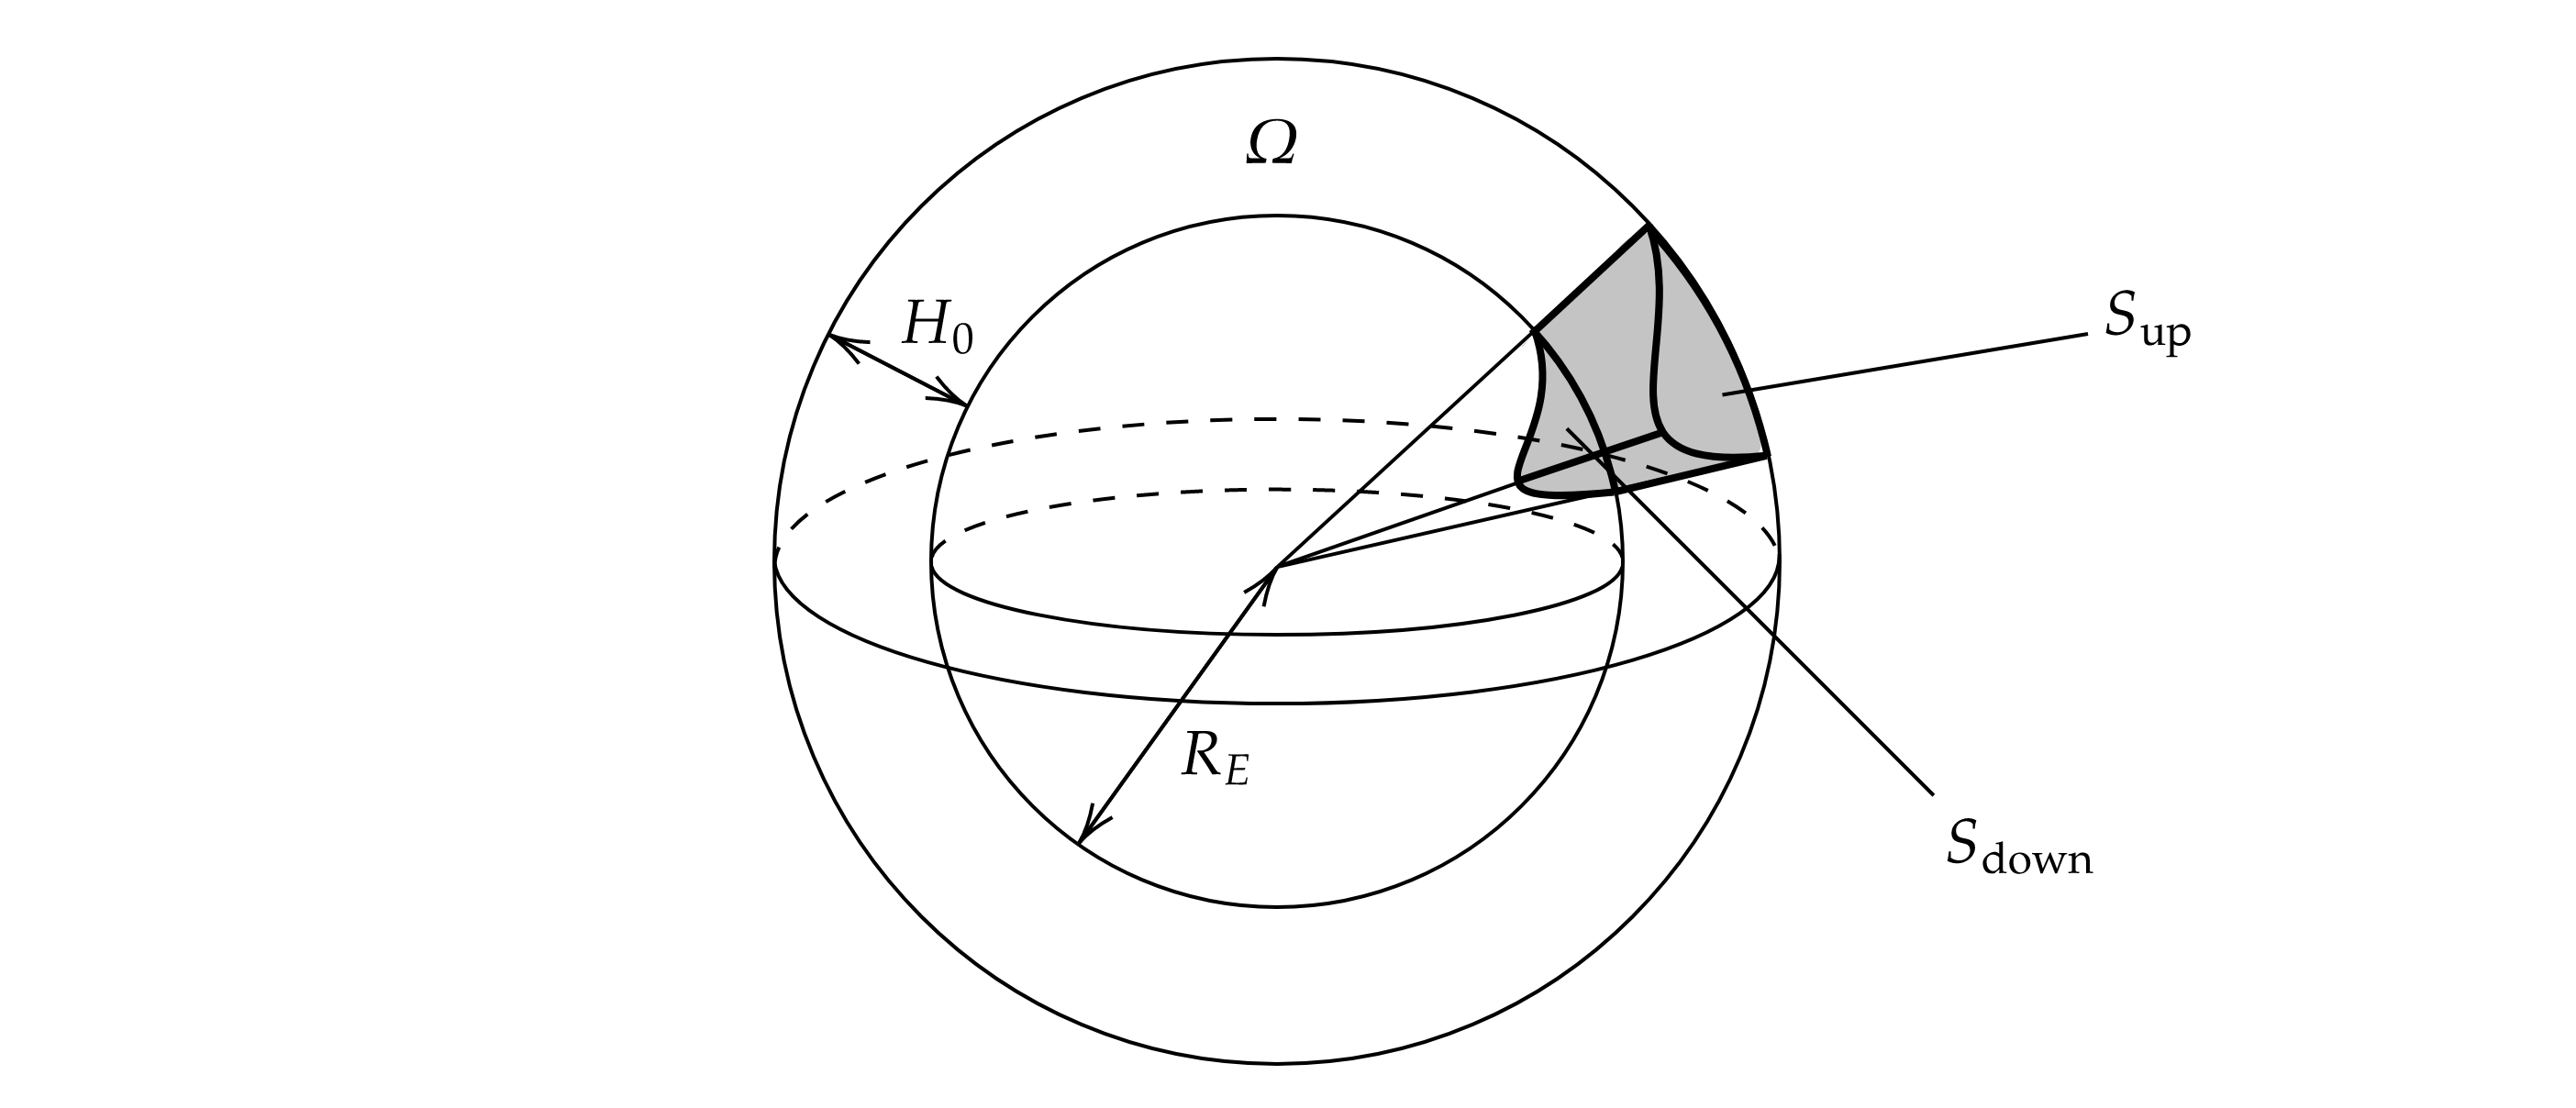
\includegraphics[width=\textwidth]{figures/konus.png}
    \caption{Примерный вид одной из маленьких областей (выделено серым), на которые разбивается область $\Omega$ в приближении сферических поверхностей $\Gamma_1$ и $\Gamma_2$.}
    \label{fig:konus}
\end{figure}

Следует заметить, что все различие между рассматриваемой моделью и столбчатой моделью сводится к различию в формах областей, на которые разбивается область $\Omega$: в данном случае это конусы, в случае столбчатой модели --- цилиндры. Главное отличие между конусами и цилиндрами заключается в том, что у первых площади верхнего и нижнего оснований различны, а у последних --- одинаковы. Для оценки того, на сколько сильно конусы отличаются от цилиндров, следует сравнить площади оснований
\begin{equation}
    \dfrac{S_\textnormal{up}}{S_\textnormal{down}} = \dfrac{\qty(R_E + H_0)^2}{R_E^2} = \qty(1 + \dfrac{H_0}{R_E})^2.
\end{equation}
Для продвижения рассуждений следует учесть, что $H_0 = 70\, \textnormal{км}$, тогда получается следующая оценка:
\begin{equation}
    \dfrac{S_\textnormal{up}}{S_\textnormal{down}} = \qty(1 + \dfrac{70}{6371})^2 \approx 1 + 2 \cdot \dfrac{70}{6371} = 1 + 2 \cdot 0.01.
\end{equation}
Отсюда следует, что такие конусы с точностью до 2\% можно полагать цилиндрами. Это доказывает справедливость рассмотрения столбчатой модели, где вместо конусов используются цилиндры.